\phantomsection
\chapter{Viola-Jones Face detection}
\label{chap:vj}

\noindent Viola-Jones algorithm is "a visual object detection framework that is capable of processing images extremely rapidly while achieving high detection rates". 3 main points characterize this algorithm. The first one is the use of what is called an "integral image", which is a new representation of the image allowing the features to be computed very quickly. Second point is the use of a learning algorithm based on AdaBoost, which builds efficient classifiers. The third and last point is the use of a method to combine classifiers. This method combine classifiers in "cascade". It allows to focus on the promising object-like regions by discarding the background in a very quick way \cite{VIO01}.
\newline

\phantomsection
\section{Overview}

\vspace{\baselineskip}
\noindent The Viola-Jones algorithm works as following \cite{DIN08}:

\begin{itemize}
  \item This algorithm is a "strong, binary classifier built of several weak detectors"
  \item "Each weak detector is a simple binary classifier"
  \item During the learning part, a cascade of weak classifiers is used and trained in order to reach the desired hit/miss rate using AdaBoost learning algorithm
  \item The input image is then divided into several rectangular sub-regions in order to detect objects. Each sub-region is computed by the cascade of classifiers;
  \item To classify a sub-region as "positive", it has to pass all stages of the cascade
  \item The algorithm iterates over the 2 last steps with sub-regions of different sizes.
\end{itemize}

\phantomsection
\section{Haar features}

\vspace{\baselineskip}
\noindent The features used by Viola and Jones are based on Haar wavelets, which are single wavelength square waves. A square wave is composed of a high interval and a low interval. In a two dimensional space, a square wave is represented by a pair of adjacent rectangles: a light one and a dark one. True Haar wavelets are however not used in rectangle combinations for visual object detection. There are better suited features for this task, which are Haar-like, hence the name of Haar (or Haar-like) features, instead of Haar wavelets \cite{HEW07}.
\newline

\noindent Figure~\ref{haar_features_first_2_stage} shows some of the first Haar features in the original Viola-Jones cascade \cite{HEW07}, while Figure~\ref{haar_features_extended} is an example from the extended set of features \cite{DIN08}. Figure~\ref{haar_features_early_stage} is an example of an early stage in the Haar cascade. In these examples, each pair of black and white rectangles represents a feature. These features are used by the algorithm to detect regions of interest in the input image \cite{HAR12}.
\newline

\begin{figure}[!h]
\begin{center}
\noindent 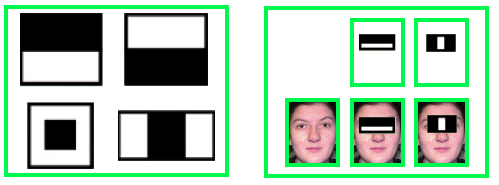
\includegraphics[scale=0.8]{figures/haar_features_first_2_stage} 
\newline
\caption{Examples Haar features}
\label{haar_features_first_2_stage}
\end{center} 
\end{figure}

\begin{figure}[!h]
\begin{center}
\noindent 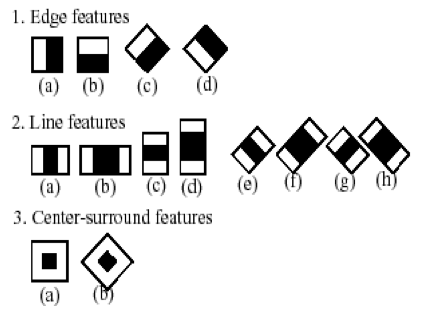
\includegraphics[scale=0.6]{figures/haar_features_extended} 
\newline
\caption{Extended set of features \cite{DIN08}}
\label{haar_features_extended}
\end{center} 
\end{figure}

\begin{figure}[!h]
\begin{center}
\noindent 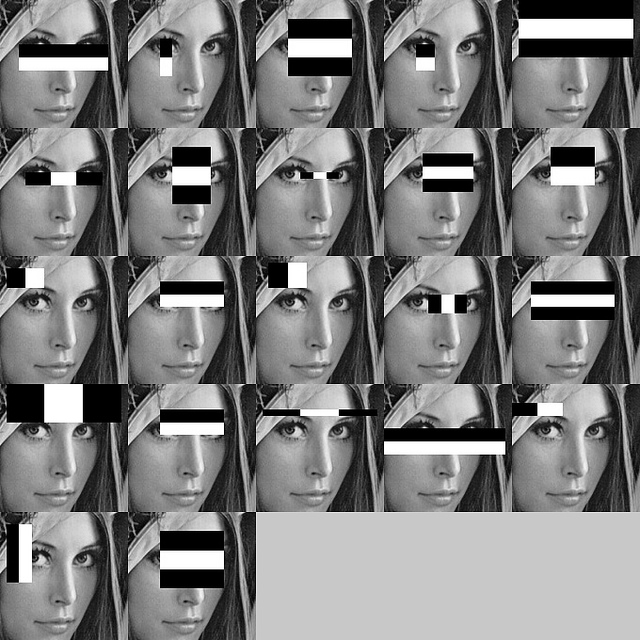
\includegraphics[scale=0.5]{figures/haar_features_early_stage} 
\newline
\caption{Example of an early stage in the Haar cascade \cite{HAR12}}
\label{haar_features_early_stage}
\end{center} 
\end{figure}

\noindent Basic subtraction is used to detect the presence of Haar features. It consists of subtracting the average pixel value of the dark region from the average pixel value of the light region. There is then a thresholding of the result, where the feature is considered present if it is above the threshold. If the outcome is positive, the current stage is validated, and the feature can go on the next stage \cite{HEW07}. There are about 20 to 30 different stages in order to detect the presence of Haar features. The first stage is a very coarse scan of the image, while following stages are more finely tuned and harder to pass \cite{HAR12}.
\newline

\noindent For example, Figure~\ref{haar_feature_later_stage} shows a later stage in the Haar cascade. Compared to an earlier stage as in Figure~\ref{haar_features_early_stage}, there are many more patterns of black and white rectangles that need to match the input image \cite{HAR12}.
\newline

\begin{figure}[!h]
\begin{center}
\noindent 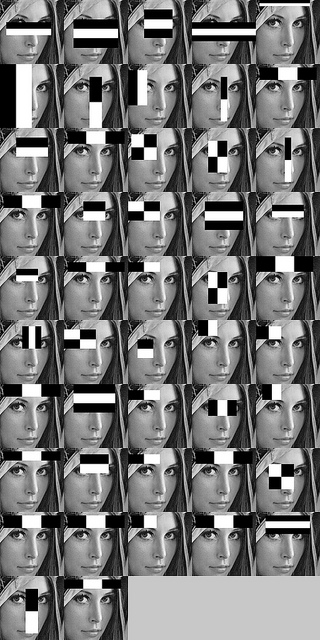
\includegraphics[scale=0.8]{figures/haar_feature_later_stage} 
\newline
\caption{Example of a later stage in the Haar cascade \cite{HAR12}}
\label{haar_feature_later_stage}
\end{center} 
\end{figure}

\noindent There are 3 kinds of features used by Viola-Jones' algorithm: a two-rectangle feature, a three-rectangle feature and a four-rectangle feature, as seen in Figure~\ref{haar_feature_description}. Indeed, images (A) and (B) show the two-rectangle features, image (C) shows the three-rectangle feature, and image (D) shows the four-rectangle feature \cite{VIO01}.
\newline

\noindent For two-rectangle features, the output value is computed by the difference between the sum of the pixels being in the two rectangular regions. The 2 regions are identical, with same size and same shape, and they are horizontally or vertically adjacent. 
\newline

\noindent The three-rectangle feature value is calculated by the sum of the pixels of the two outside rectangles subtracted from the sum of the pixels in the central rectangle. 
\newline

\noindent The last kind of feature is the four-rectangle feature, which value consists in the difference between the diagonal pairs of rectangles \cite{VIO01}.
\newline

\begin{figure}[!h]
\begin{center}
\noindent 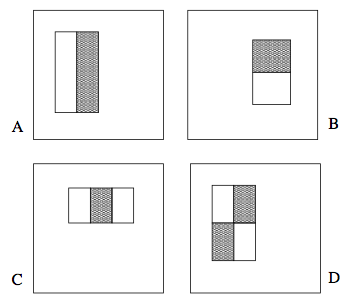
\includegraphics[scale=0.6]{figures/haar_feature_description} 
\newline
\caption{Example of the different kinds of rectangle features}
\label{haar_feature_description}
\end{center} 
\end{figure}

\noindent Viola and Jones admit that rectangle features can be considered as primitive features. In contrast with other features, rectangle features are quite coarse, even though they are sensitive to the presence of edges, bars and other simple image structure. It however appears that a rich image representation is provided by this set of rectangle features, and this representation supports effective learning. Compared to the great computational efficiency provided by rectangle features, their limited flexibility is then not much of a problem \cite{VIO01}.
\newline

\phantomsection
\section{Integral image}

\vspace{\baselineskip}
\noindent Viola and Jones used an intermediate representation of an image called "integral image". This integral image allows a very fast computation of rectangle features \cite{VIO01}, which then influences the determination of the presence or absence of hundreds of Haar features. In general, adding small units together is similar to integrating them; here, the small units are pixel intensity values. The integral value of a pixel can hence be computed by summing values from pixels above it and on its left. Integration of an entire image consequently starts at the top left corner and goes through all the image to the down right corner \cite{HEW07}.
\newline

\noindent For a pixel P with coordinates ($x,y$), its value in the integral image is computer as follows: \[ ii(x,y) = \sum_{x' \leq x,y' \leq y} i(x',y') \] where $ ii(x,y) $ is the integral image and $ i(x,y) $ is the input image intensity value function. In Figure~\ref{integral_image_description}, the value of the integral image at point $ (x,y) $ is represented as the sum of all pixels above and on its left \cite{VIO01}. 
\newline
	
\begin{figure}[!h]
\begin{center}
\noindent 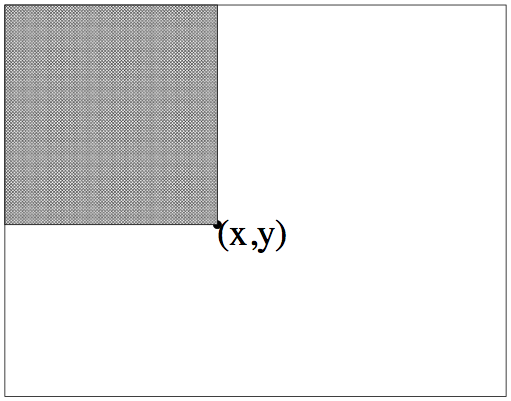
\includegraphics[scale=0.5]{figures/integral_image_description} 
\newline
\caption{Integral image}
\label{integral_image_description}
\end{center} 
\end{figure}
	
\noindent Using the following pair of recurrences: 
\begin{equation}
s(x,y) = s(x,y - 1) + i(x,y)
\end{equation}
\begin{equation}
ii(x,y) = ii(x - 1,y) + s(x,y)
\end{equation}
(where $ s(x,y) $ is the cumulative row sum, $ s(x,-1) = 0 $, and $ ii(-1,y) = 0 $) the integral image can be computed in only one pass over the original image. 
\newline

\noindent In Figure~\ref{integral_image_four_array}, the sum of the pixels in rectangle D can be calculated with four array references, thanks to the integral image. Value of the integral image at point 1 is the sum of pixels in rectangle $ A $. Value at point 2 is $ A + B $, at point 3 is $ A + C $, and at  point 4 is $ A + B + C + D $. The sum in D can then be computed as $ 4 + 1 - (2 + 3) $ \cite{VIO01}. 
\newline

\begin{figure}[!h]
\begin{center}
\noindent 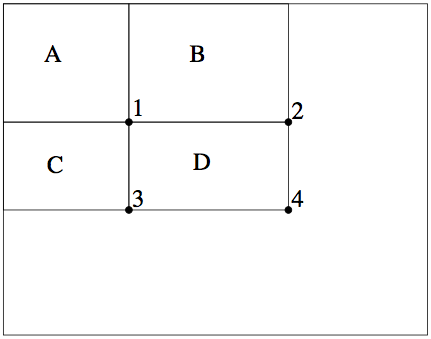
\includegraphics[scale=0.6]{figures/integral_image_four_array} 
\newline
\caption{Integral image with four array references}
\label{integral_image_four_array}
\end{center} 
\end{figure}

\phantomsection
\section{Weak classifiers and AdaBoost}

\vspace{\baselineskip}
\noindent Features are extracted from a sub-region of an input image, which size is usually of $ 24\times24 $ pixels. Each feature type is moved and scaled across the entire input image, which means that there are about 160,000 possible combinations to process in a 24 pixel by 24 pixel sub-region \cite{SMY07}.
\newline

\noindent AdaBoost is a machine-learning method used by Viola and Jones in order to select specific Haar features to use. It is also used to set the threshold levels. This method is based on the statement that the combination of many weak classifiers forms a strong one. They are called weak classifiers because their accuracy and efficiency are only a bit above random guessing, which is not particularly good. The purpose of using so many weak classifiers is to get a right answer with a higher rate of success. This algorithm relies on on the verified hypothesis that if each weak classifier pushes the final answer a little bit in the right direction each time, it means the correct answer will be obtained in the end \cite{HEW07}. 
\newline

\noindent AdaBoost works the following way: it chooses a set of weak classifiers that are going to be combined and assigns a weight to each classifier (see Figure~\ref{haar_feature_adaboost}). The result of this weighted combination is a strong classifier \cite{HEW07}. One of the difficulties and challenges for this learning algorithm is to associate large weights to efficient classifiers, and smaller weights toeach poor classifiers. In order to succeed in selecting a small group of good classifiers but with significant variety, AdaBoost is an aggressive algorithm \cite{VIO01}.
\newline

\begin{figure}[!h]
\begin{center}
\noindent 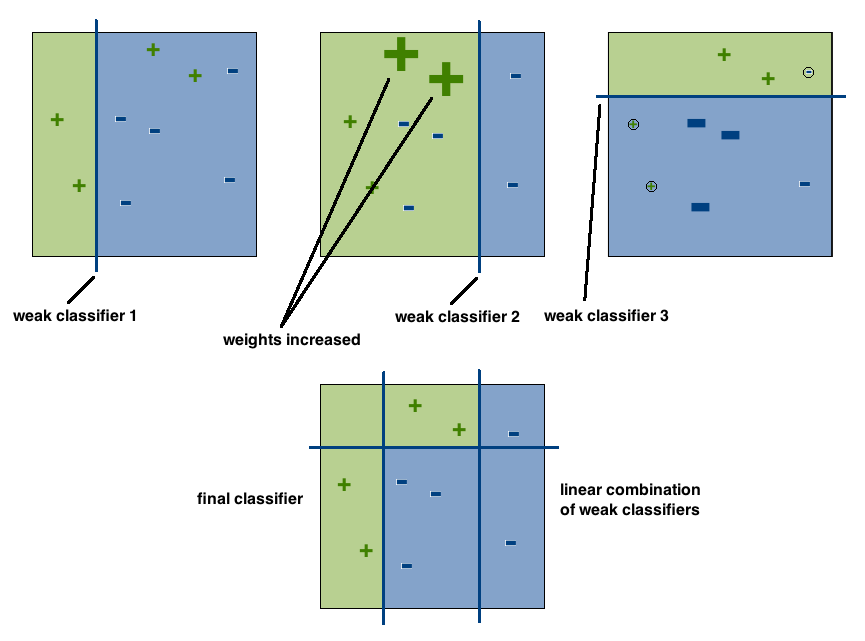
\includegraphics[scale=0.6]{figures/haar_feature_adaboost} 
\newline
\caption{AdaBoost method}
\label{haar_feature_adaboost}
\end{center} 
\end{figure}

\noindent Experiments have been conducted with a classifier built from 200 features and using AdaBoost. The classifier had a detection rate of 95\%, and obtaind only 1 false positive out of 14084 negative samples from the training dataset (see figure~\ref{haar_feature_example_result}) \cite{VIO01}.
\newline

\begin{figure}[!h]
\begin{center}
\noindent 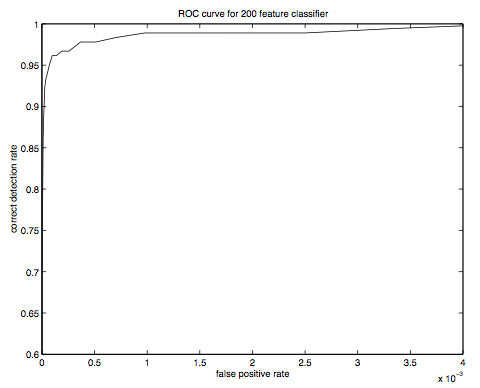
\includegraphics[scale=0.8]{figures/haar_feature_example_result} 
\newline
\caption{Receiver Operating Characteristic (ROC) curve for the 200 feature classifier \cite{VIO01}}
\label{haar_feature_example_result}
\end{center} 
\end{figure}

\noindent This experiment, points out that a 200-feature classifier is an efficient technique for object detection. It also means that a boosted classifier constructed from rectangle features is an efficient technique for object detection. Although the results of this experiment are convincing in terms of detection, they may not be performant enough for real-world tasks. This boosted classifier requires 0.7 seconds to scan a $ 384\times288 $ pixel image. Regarding the computation time, it is probably faster than any other existing system. In order to improve the system so that it will perform well in real-world conditions, detection performance must be improved. The most straightforward method to achieve that is to add features to the classifier. Doing that will immediately decrease the speed of this system; it will increase computation time \cite{VIO01}.
\newline

\phantomsection
\section{Classifiers cascade}

\vspace{\baselineskip}
\noindent What Viola and Jones did to classify image regions and sub-regions in an efficient way is to combine AdaBoost classifiers as a filter chain. It is constructed as a cascade a hence its name  "Classifiers cascade". This chain is composed of a separate AdaBoost classifier for each filter, which has a fairly small number of weak classifiers. As in figure~\ref{haar_feature_cascade}, the classifier cascade represents a chain of filters. If an image sub-region passes successfully all cascade steps, it is labelled as "Face", otherwise it is classified as "Not Face" \cite{HEW07}. Using this algorithm with the classifiers cascade method allows to reduce significantly the computation time and increase significantly the detection performance \cite{VIO01}.
\newline

\begin{figure}[!h]
\begin{center}
\noindent 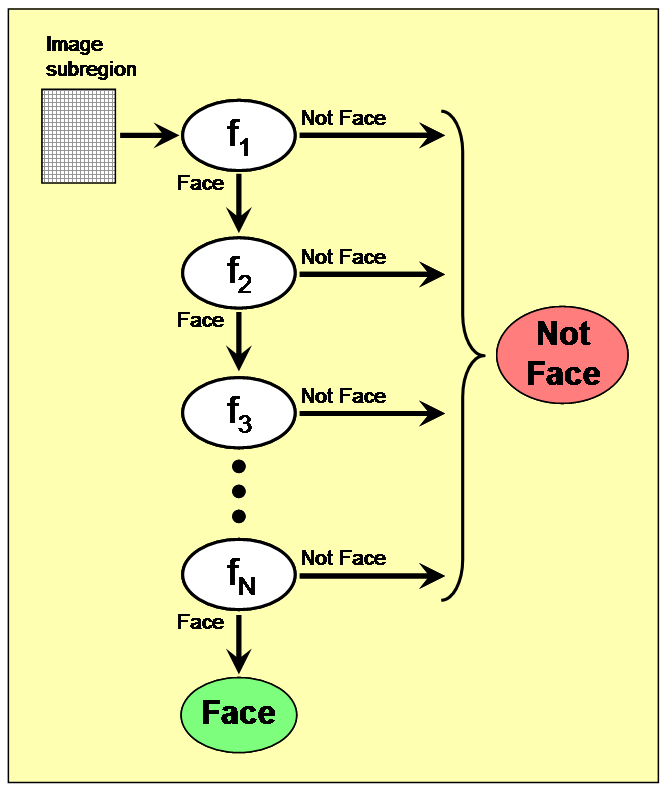
\includegraphics[scale=0.5]{figures/haar_feature_cascade} 
\newline
\caption{Cascade of boosted classifiers}
\label{haar_feature_cascade}
\end{center} 
\end{figure}

\noindent Tests were conducted to see if the cascade method was feasible. Two simple detectors were trained, one of them being a 200-feature classifier and the other one being a cascade of 10 20-feature classifiers. Figure~\ref{haar_feature_cascade_example_result} gives the ROC curves comparing the two classifiers' performance. Between the two classifiers, regarding their accuracy, the difference is little and not significant. On the other hand, regarding their speed, the difference is large and significant, the classifier cascade being about 10 times faster. This is because as soon as the first stage, most negative samples are discarded, so they will not be evaluated ever again afterwards \cite{VIO01}.
\newline

\begin{figure}[!h]
\begin{center}
\noindent 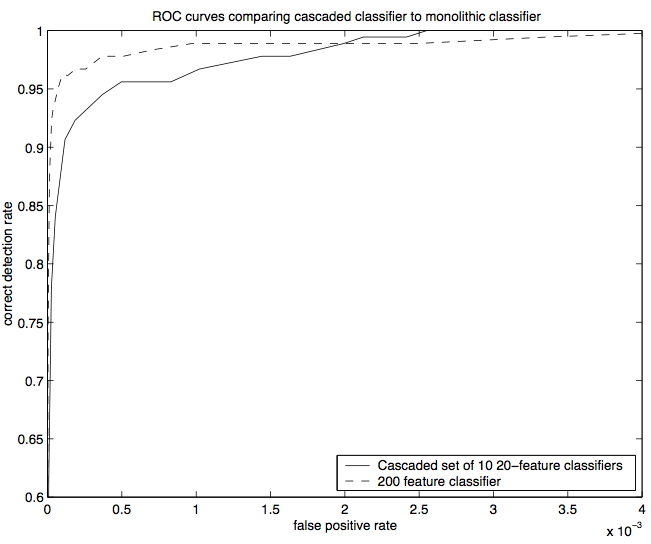
\includegraphics[scale=0.6]{figures/haar_feature_cascade_example_result} 
\newline
\caption{ROC curves of a 200-feature classifier and of a classifier cascade containing 10 20-feature classifiers \cite{VIO01}}
\label{haar_feature_cascade_example_result}
\end{center} 
\end{figure}

\noindent The cascade method has been made in a way that there must not be false negative labeling, meaning that no face should be classified as "Not Face". The assistance threshold has been set low for each level, low enough for the training set to pass all or almost all face examples. All training images that passed previous stages are classified by filters trained to do it for each level. A region is immediately classified as "Not Face" as soon as it failed at one filter. If one of these filters succeeds to pass a region, then it is up to the next filter in the chain. If a region succeed to pass through all the filters present in the chain, then it can be classified as "Face" \cite{HEW07}.
\newline

\noindent The key point of this method is to construct smaller, more efficient, boosted classifiers. They will then detect nearly all positive instances while rejecting a lot of negative sub-regions. Before using complex classifiers to achieve low false positive rates, simple classifiers are called to reject most sub-regions \cite{VIO01}.
\newline

\noindent The order of the filters in the cascade is not random; it is based on the importance weighting assigned by AdaBoost. Heavily weighed are called early, so they eliminate non-face sub-regions as soon as possible. Figure~\ref{haar_feature_first_2_features} shows the first 2 features from Viola-Jones cascade, applied to a face. The first feature used is the one with the eye region being darker than the cheek region. The second feature used is the one with the eyes region being darker than the bridge of the nose \cite{HEW07}.
\newline

\begin{figure}[!h]
\begin{center}
\noindent 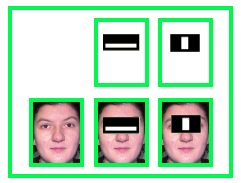
\includegraphics[scale=1]{figures/haar_feature_first_2_features} 
\newline
\caption{The first two Haar features in the original Viola-Jones cascade}
\label{haar_feature_first_2_features}
\end{center} 
\end{figure}

\noindent The structure of the cascade in itself means that within any single image, most sub-regions are negative. The cascade hence tries to reject as many negatives as possible, starting at the first stage. Indeed, when a positive instance occurs, it will trigger the evaluation of all the classifiers of the cascade, which can be time consuming \cite{VIO01}.
\newline

\noindent Following are the different numbers about cascade classifiers (see Figure~\ref{haar_feature_cascade_rate}) \cite{UBC01}:

\begin{itemize}
  \item 1-feature classifier: 100\% detection rate and 50\% false positive rate
  \item 5-features classifier: 100\% detection rate and 40\% false positive rate 
  \item 20-features classifier: 100\% detection rate and 10\% false positive rate
\end{itemize}

\begin{figure}[!h]
\begin{center}
\noindent 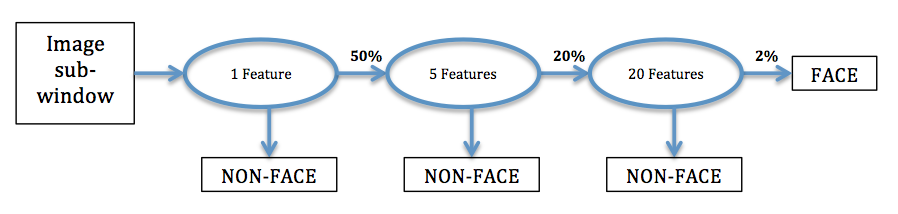
\includegraphics[scale=0.5]{figures/haar_feature_cascade_rate} 
\newline
\caption{Cascade of boosted classifiers positive rate}
\label{haar_feature_cascade_rate}
\end{center} 
\end{figure}

\phantomsection
\section{Test set and training}

\vspace{\baselineskip}
\noindent The training set is made of about 5000 hand-labelled images of faces. All faces are scaled and have the same resolution of $ 24\times24 $ pixels. All these faces were chosen randomly on the internet. Some face examples are shown in figure~\ref{haar_feature_training_dataset} \cite{VIO01}.
\newline

\begin{figure}[!h]
\begin{center}
\noindent 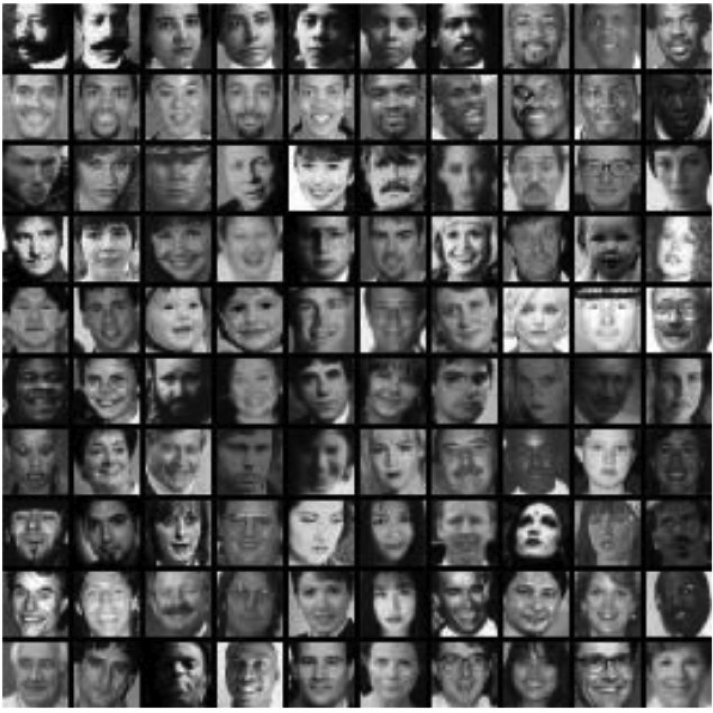
\includegraphics[scale=0.9]{figures/haar_feature_training_dataset} 
\newline
\caption{Examples of frontal upright face images used for training}
\label{haar_feature_training_dataset}
\end{center} 
\end{figure}

\noindent To sum up, the training set is composed of \cite{UBC01}:

\begin{itemize}
  \item about 5,000 faces
  \begin{itemize}
  	\item All frontal
  \end{itemize}
  \item 300 million non faces sub-regions
  \begin{itemize}
  	\item from 9,400 non-face images
  \end{itemize}
  \item Normalized faces
  \begin{itemize}
  	\item Scale, translation
  \end{itemize}
  \item Many variations
  \begin{itemize}
  	\item Between individuals
	\item Lightning
	\item Pose (rotation of the head)
  \end{itemize}
\end{itemize}

\vspace{\baselineskip}
\noindent There are usually two parts into a test set, first part being training set and second part being validation set. The training set is typically made of about 5,000 positives samples (faces) and 10,000 negative samples (non-faces, usually non-face sub-regions chosen from non-face images) \cite{DIN08}. For this kind of training, and with a 32 layer classifier, the total time usually exceeds several weeks \cite{VIO01}.
\newline

\noindent Viola-Jones training stage proceeds with the following step \cite{DIN08}:

\begin{itemize}
  \item With a defined number K of features (about 160,000 for a $ 24\times24 $ grayscale image)
  \item The number L of wanted stages has to be fixed for the cascade
  \item Then it has to be done over and over again until the number L weak classifiers is reached:
  \begin{itemize}
  	\item With the data that has be weighted again in the previous stage
	\item all the number K of weak classifiers have to be trained (the best threshold has to be find to classify in the best way the training set)
	\item The best classifier has to be chosen at this stage
	\item The data is then weighted again
  \end{itemize}
\end{itemize}

\noindent As said previously, depending on the efficiency of a weak classifier, a weight is associated to it, depending on its classification error rate. Weak classifiers are then linearly combined depending on these weights, this operation having a huge computational cost \cite{DIN08}.
\newline





